% $Header$

\documentclass{beamer}

\mode<presentation>
{
  \usetheme{default}
  \setbeamercovered{transparent}
}


\usepackage[english]{babel}

\usepackage[latin1]{inputenc}

\usepackage{times}
\usepackage[T1]{fontenc}
\usepackage{subfig}

\graphicspath{{../figures/}}

\title
{Evaluation of an Appearance-Preserving Mesh Simplification Scheme}

\author
{Rasmus Hedin}

\institute[Link�pings Universitet]
{
  Department of Electrical Engineering\\
  Link�pings Universitet
}

\date
{2018-06-15}


% If you have a file called "university-logo-filename.xxx", where xxx
% is a graphic format that can be processed by latex or pdflatex,
% resp., then you can add a logo as follows:

\pgfdeclareimage[height=0.5cm]{university-logo}{../figures/liu_primary_black_sv.pdf}
\logo{\pgfuseimage{university-logo}}



% Delete this, if you do not want the table of contents to pop up at
% the beginning of each subsection:
\AtBeginSubsection[]
{
  \begin{frame}<beamer>{Outline}
    \tableofcontents[currentsection,currentsubsection]
  \end{frame}
}


% If you wish to uncover everything in a step-wise fashion, uncomment
% the following command: 

%\beamerdefaultoverlayspecification{<+->}


\begin{document}
\captionsetup[subfloat]{labelformat=empty}

\begin{frame}
  \titlepage
\end{frame}

\begin{frame}{Outline}
  \tableofcontents
  % You might wish to add the option [pausesections]
\end{frame}


% Since this a solution template for a generic talk, very little can
% be said about how it should be structured. However, the talk length
% of between 15min and 45min and the theme suggest that you stick to
% the following rules:  

% - Exactly two or three sections (other than the summary).
% - At *most* three subsections per section.
% - Talk about 30s to 2min per frame. So there should be between about
%   15 and 30 frames, all told.

\section{Introduction}

\subsection[Short First Subsection Name]{First Subsection Name}

\begin{frame}{Make Titles Informative. Use Uppercase Letters.}{Subtitles are optional.}
  \begin{itemize}
  \item Item 1

  \item Item 2

  \end{itemize}
\end{frame}


\subsection{Second Subsection}

\begin{frame}{Make Titles Informative.}
\end{frame}

\begin{frame}{Make Titles Informative.}
\end{frame}

\section{Implementation}
% == Figures ==
% mesh transformations
% plane point distance
% qem
% quadric planes
% wedge vertex
% pyramid
% pull filter
% push filter

\section{Evaluation}
% == Figures ==
% rhombicuboctahedron
% volume


\section{Results}
% luminance
\begin{frame}{Rms Luminance Error}
  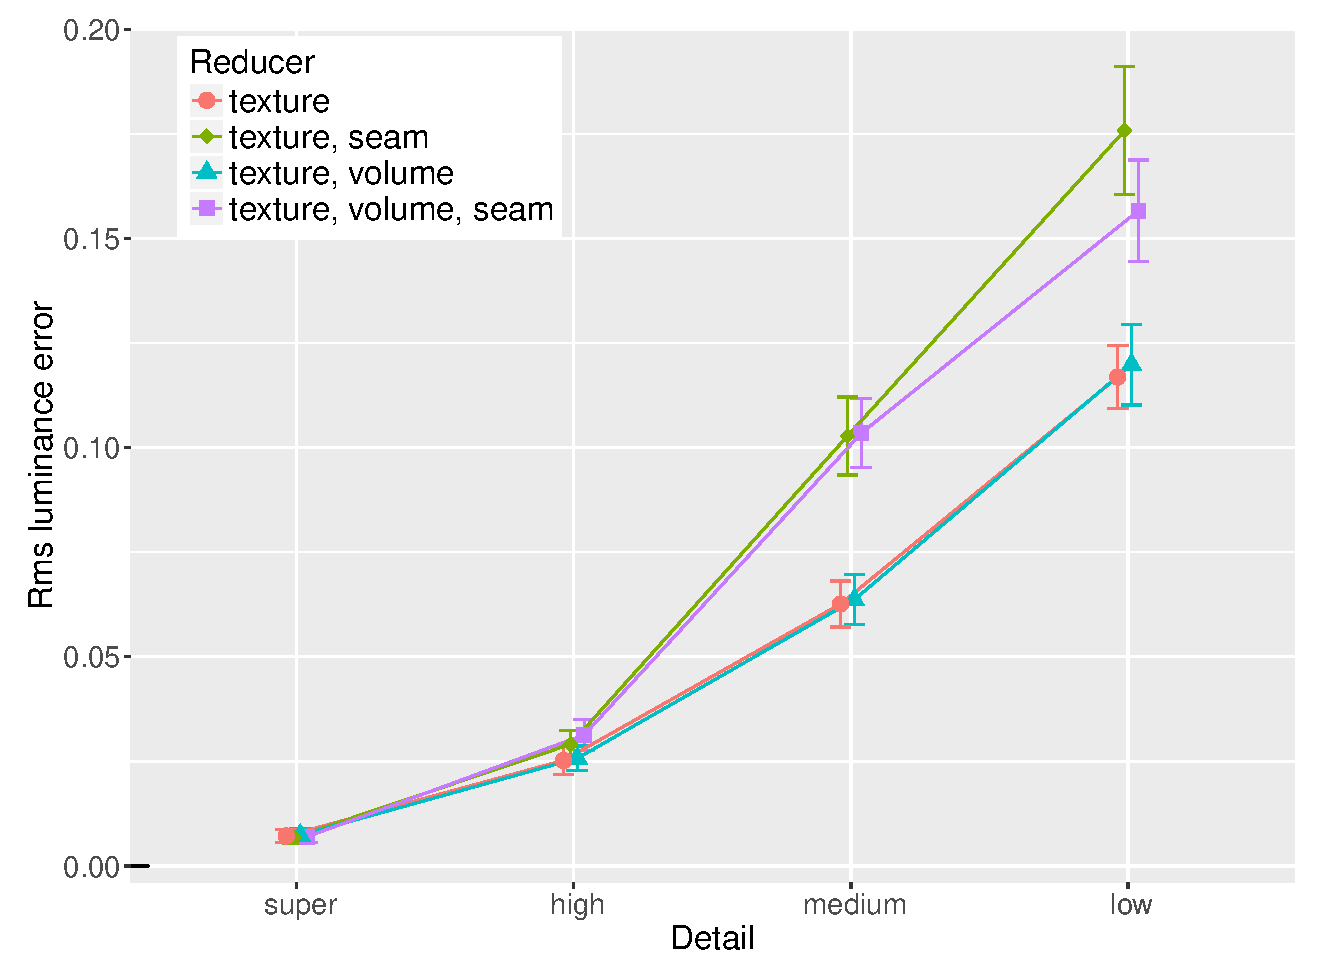
\includegraphics[width=.9\linewidth]{Rdata/rms_luminance.eps}
\end{frame}
  
% color and geometry
\begin{frame}{Geometric Error}
  \begin{figure}
    \subfloat[Rms geometric error]{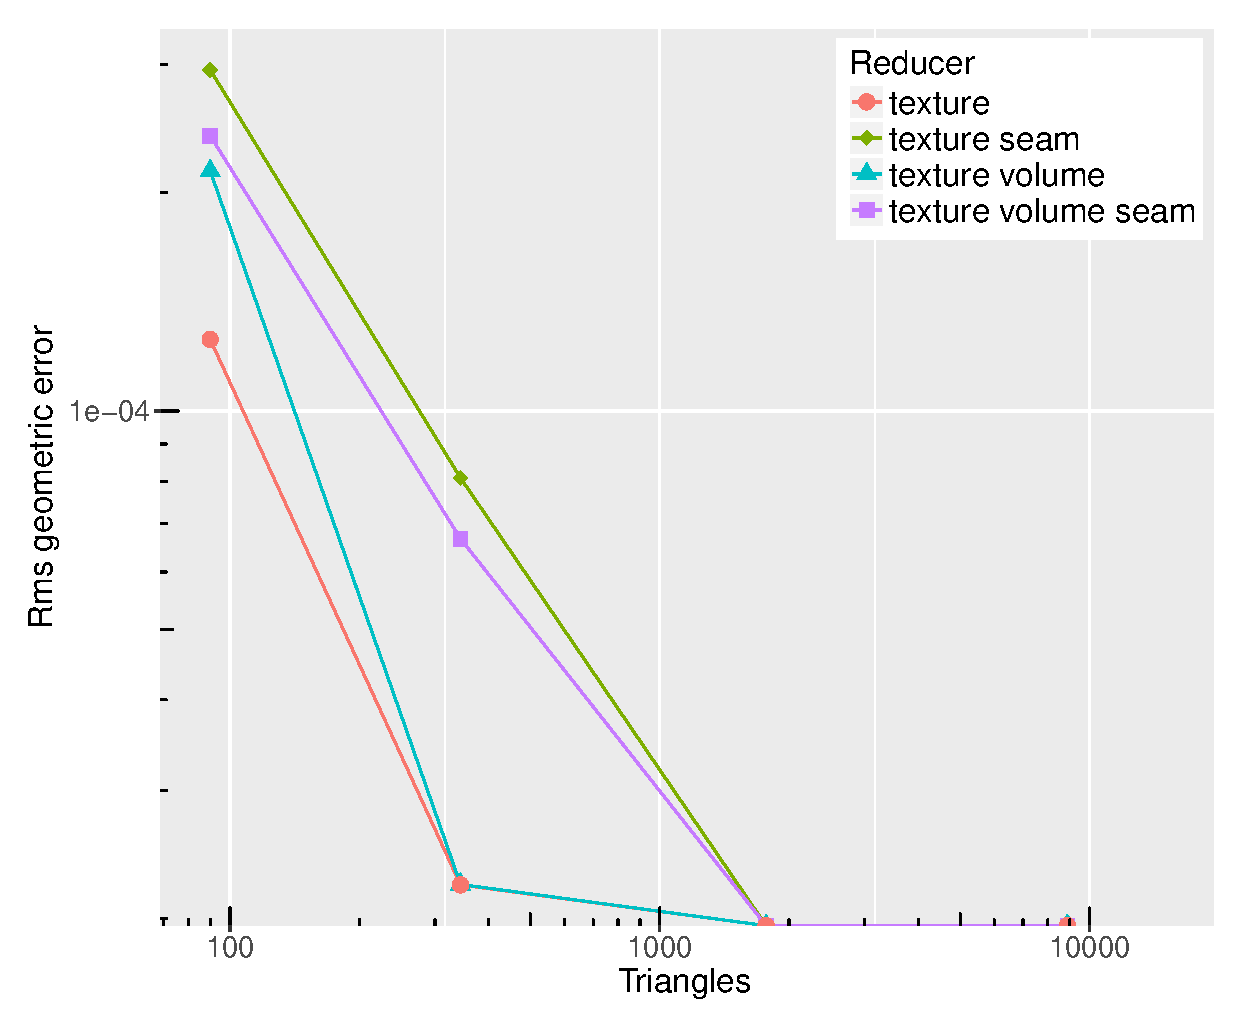
\includegraphics[width=.5\linewidth]{Rdata/rms_geometric_800.eps}}
    \subfloat[Max geometric error]{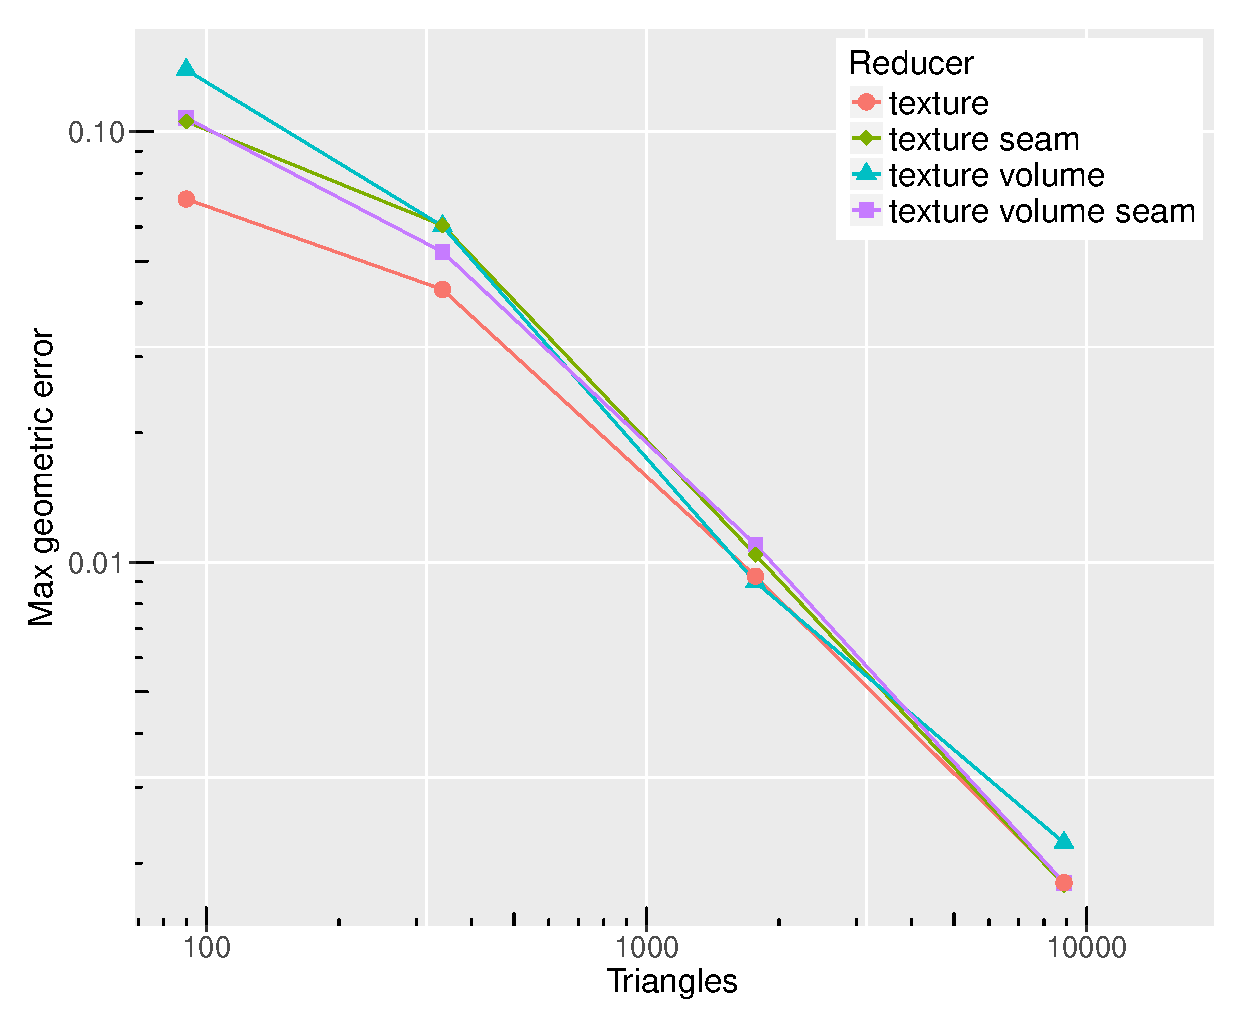
\includegraphics[width=.5\linewidth]{Rdata/max_geometric_800.eps}}
  \end{figure}
\end{frame}

\begin{frame}{Color error}
  \begin{figure}
    \subfloat[Rms color error]{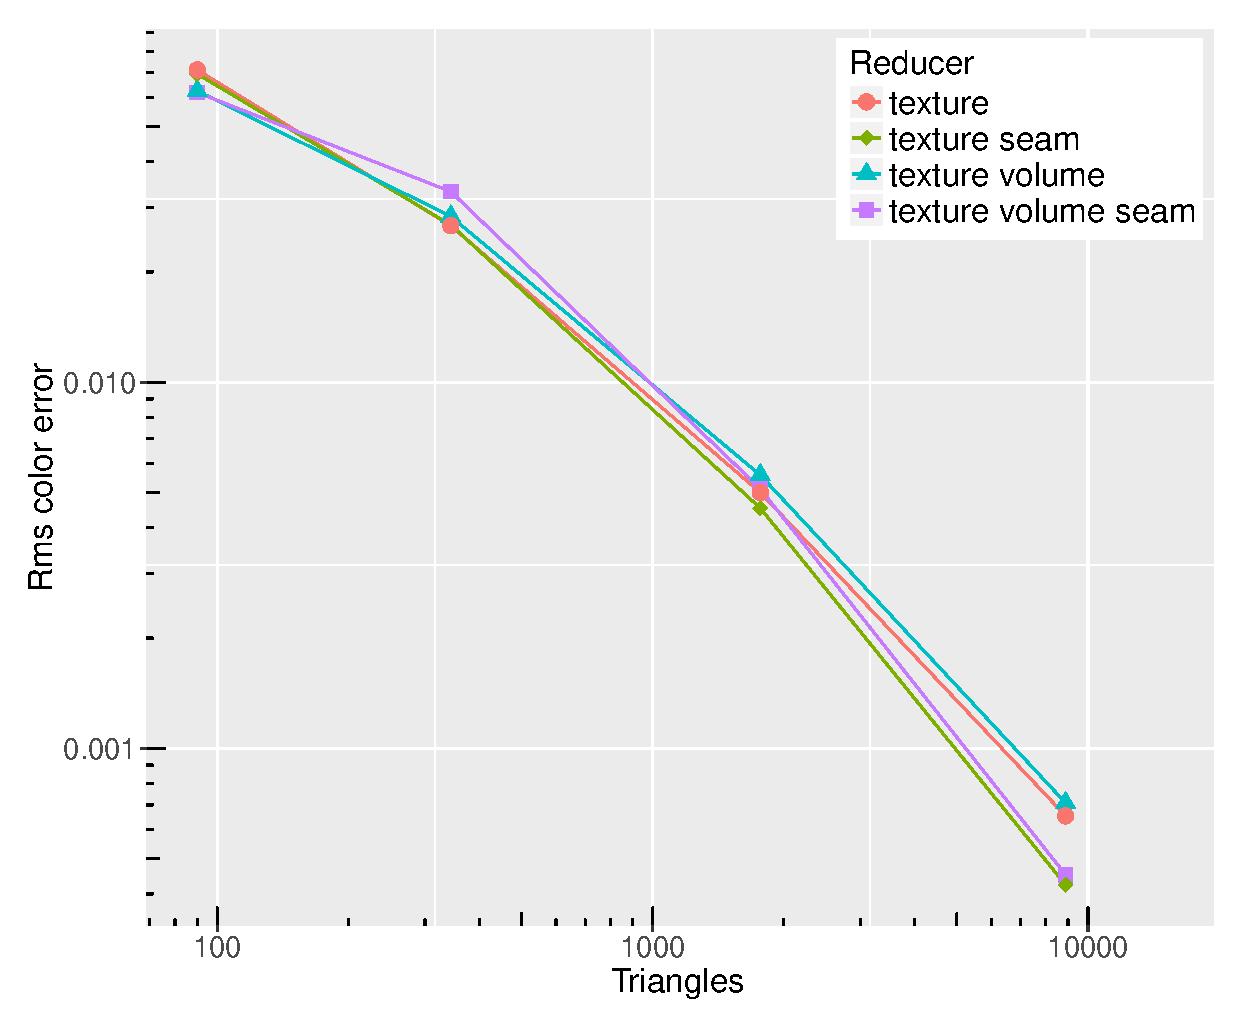
\includegraphics[width=.45\linewidth]{Rdata/rms_color_800.eps}}
    \subfloat[Max color error]{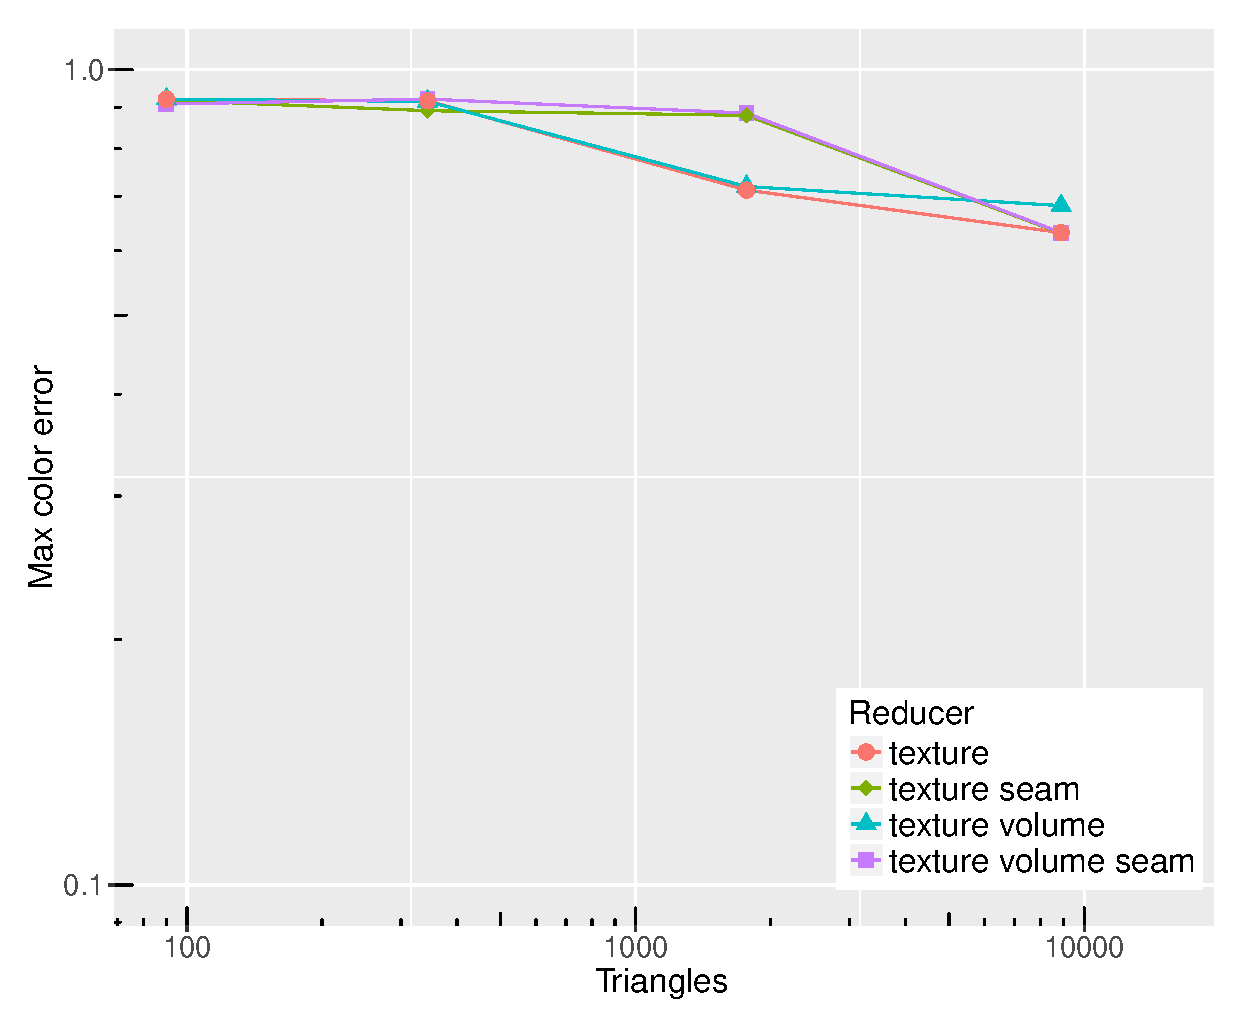
\includegraphics[width=.45\linewidth]{Rdata/max_color_800.eps}}
  \end{figure}
\end{frame}

% volume
\begin{frame}{Volume}
  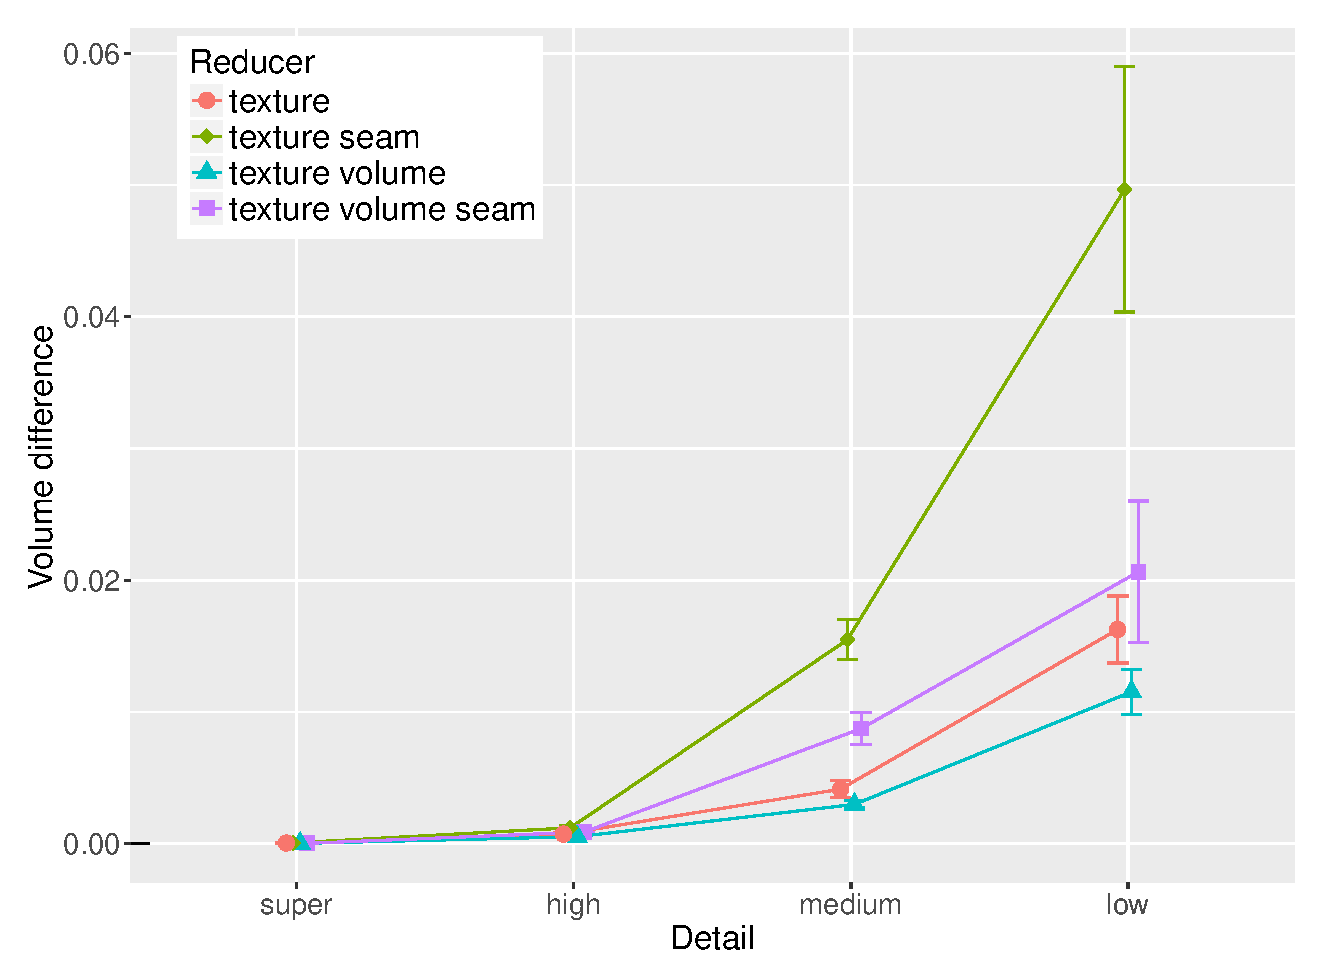
\includegraphics[width=.9\linewidth]{Rdata/volume_diff.eps}
\end{frame}

\begin{frame}{Execution Time}
  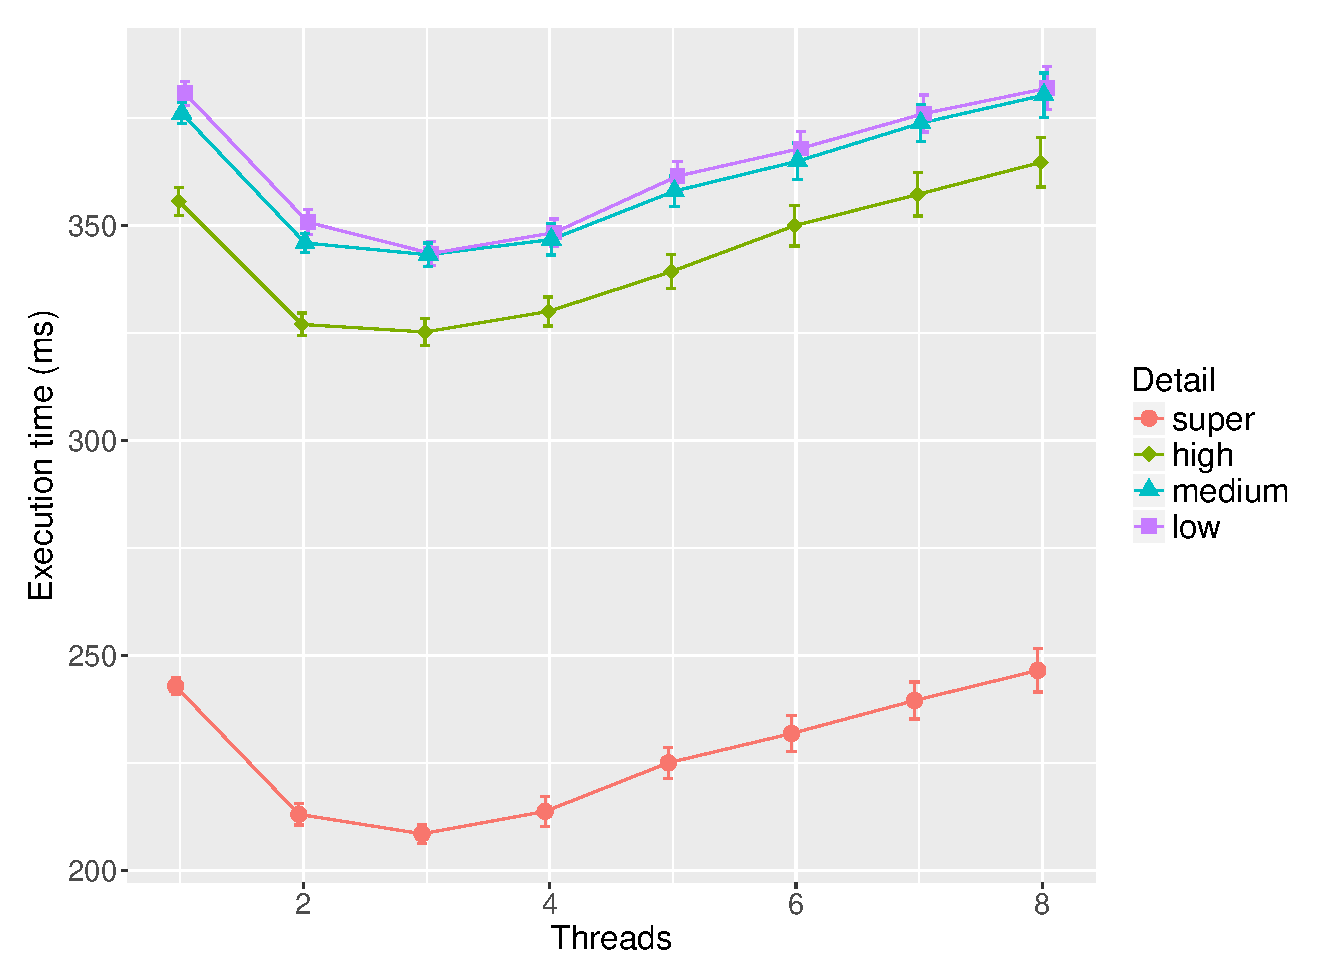
\includegraphics[width=.9\linewidth]{Rdata/parallel_execution_time.eps}
\end{frame}

% texture repair
\begin{frame}{Improving Texture}
  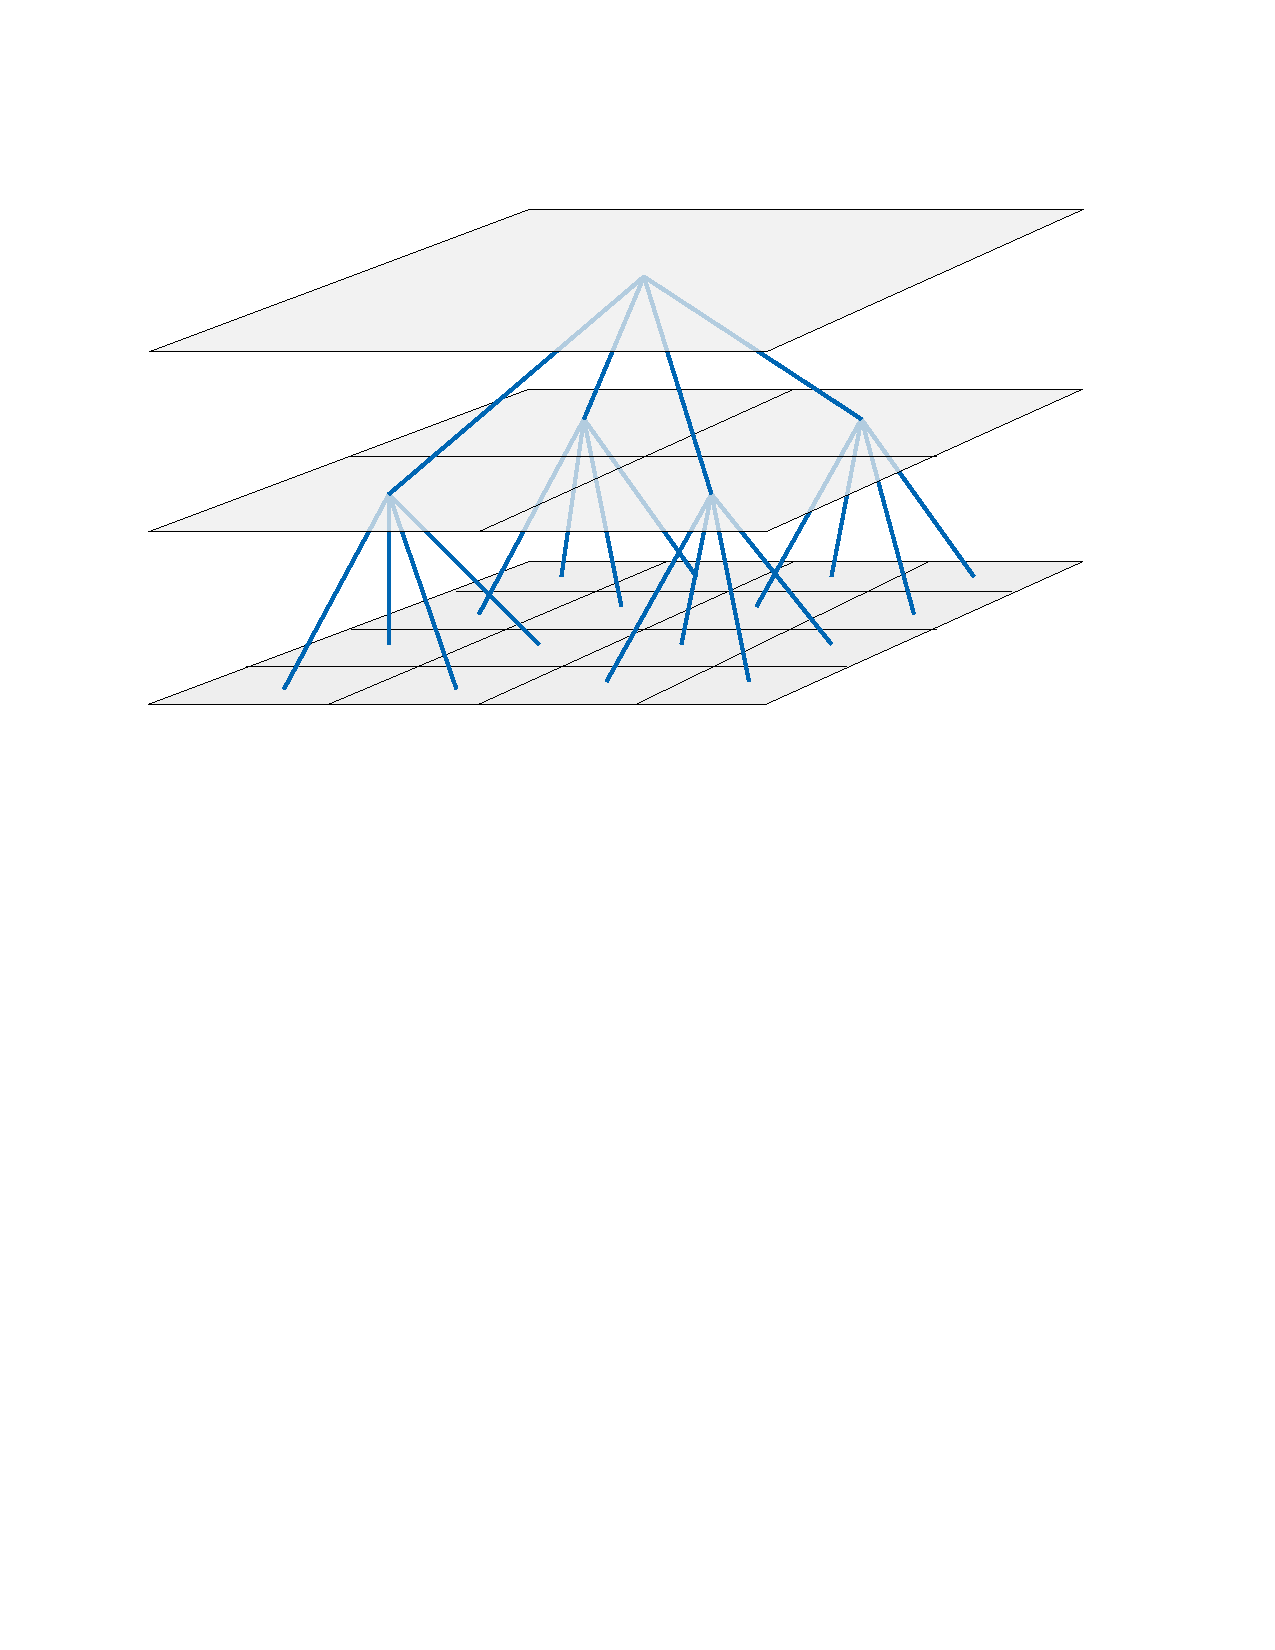
\includegraphics[width=.9\linewidth]{pyramid.pdf}
\end{frame}


\begin{frame}{Improving Texture}
  \begin{figure}
    \subfloat[Original]{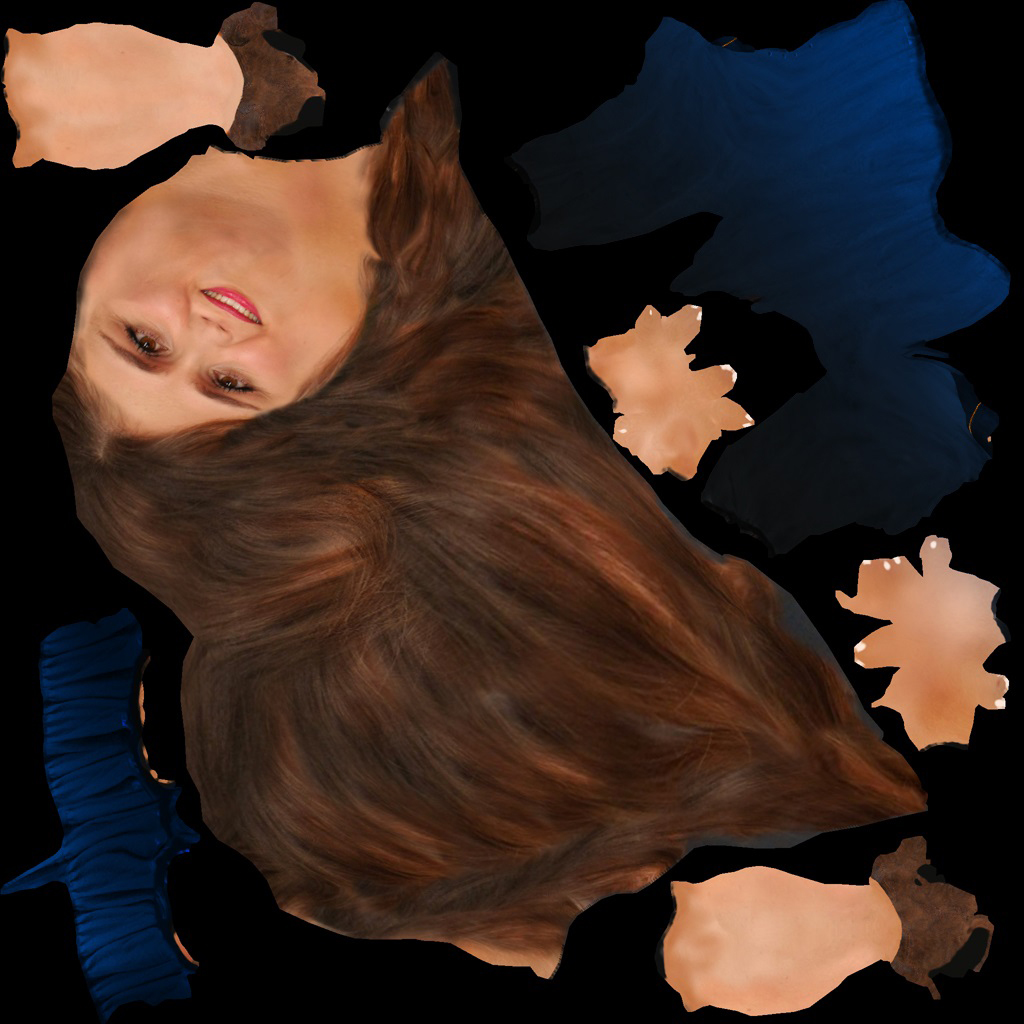
\includegraphics[width=.3\linewidth]{woman_input.jpg}}
    ~
    \subfloat[Bound]{
\includegraphics[width=.3\linewidth]{woman_bound.png}}
    ~
    \subfloat[Improved]{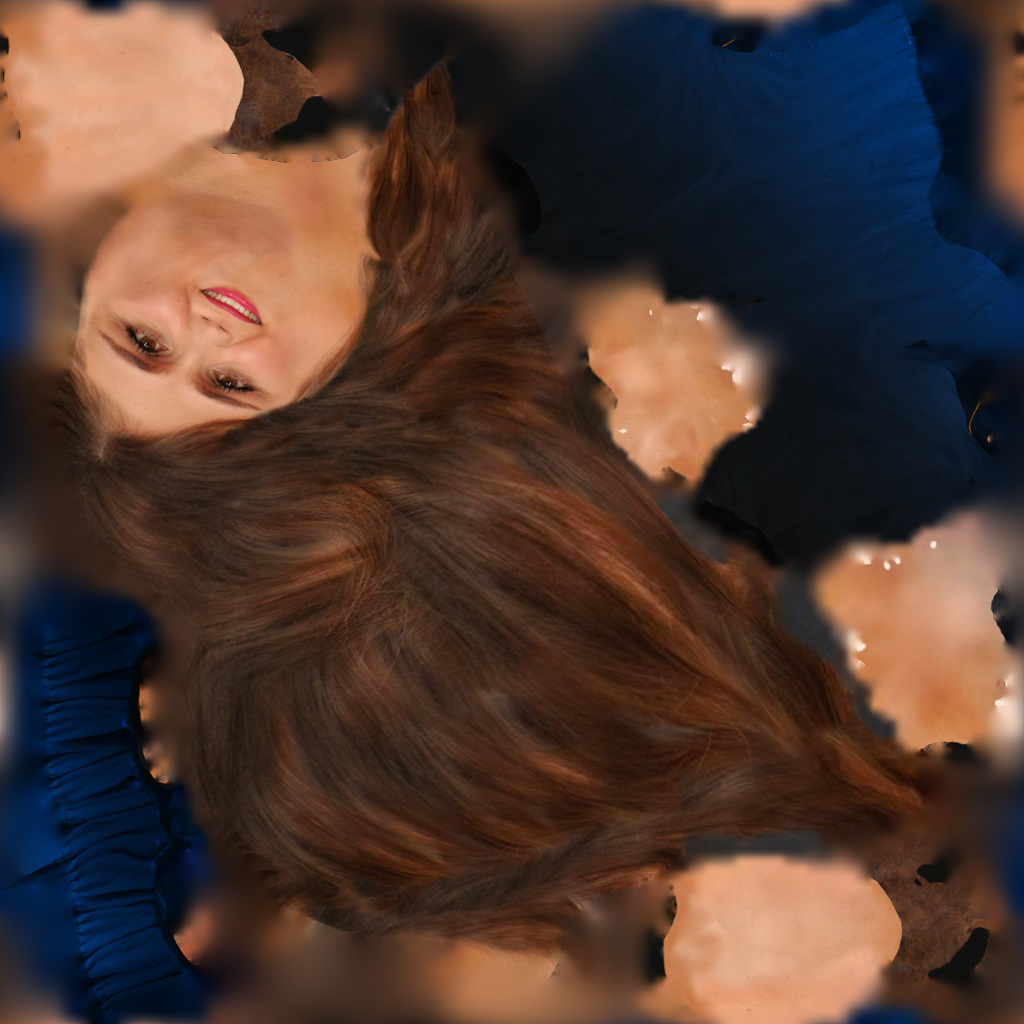
\includegraphics[width=.3\linewidth]{woman_output.png}}
  \end{figure}
\end{frame}

\begin{frame}{Improving Texture}
  \begin{figure}
    \subfloat{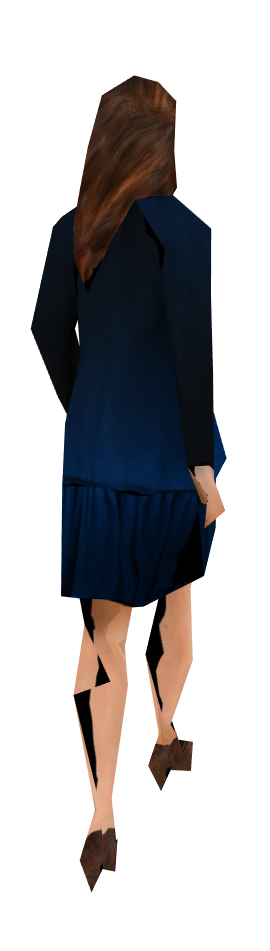
\includegraphics[width=.2\linewidth]{woman_render.png}}
    ~~~~
    \subfloat{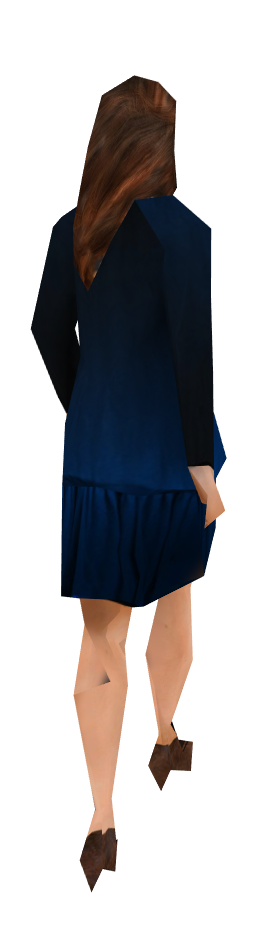
\includegraphics[width=.2\linewidth]{woman_render_improved.png}}
  \end{figure}
\end{frame}

\begin{frame}{LoD:s (only geometry)}
  \begin{figure}
    \subfloat[Super]{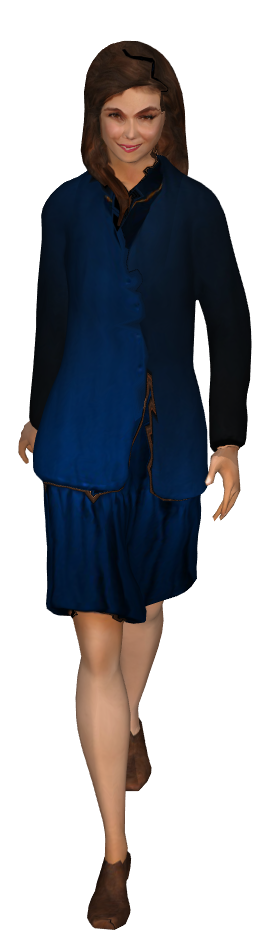
\includegraphics[width=.2\linewidth]{woman/no_texture/equal_distance/1.png}}
    ~
    \subfloat[High]{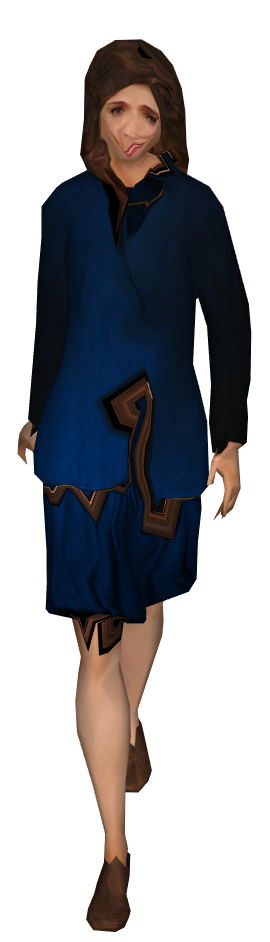
\includegraphics[width=.2\linewidth]{woman/no_texture/equal_distance/2.png}}
    ~
    \subfloat[Medium]{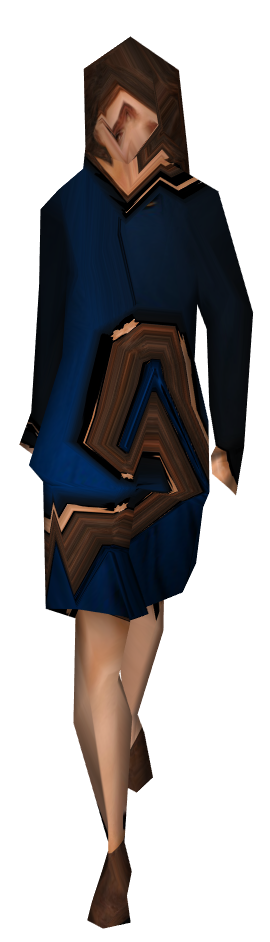
\includegraphics[width=.2\linewidth]{woman/no_texture/equal_distance/3.png}}
    ~
    \subfloat[Low]{
\includegraphics[width=.2\linewidth]{woman/no_texture/equal_distance/4.png}}
  \end{figure}
\end{frame}

\begin{frame}{LoD:s (geometry and texture)}
  \begin{figure}
    \subfloat[Super]{\includegraphics[width=.2\linewidth]{woman/equal_distance/1.png}}
    ~
    \subfloat[High]{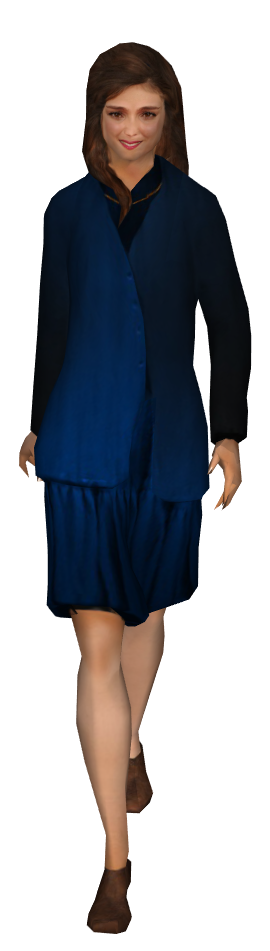
\includegraphics[width=.2\linewidth]{woman/equal_distance/2.png}}
    ~
    \subfloat[Medium]{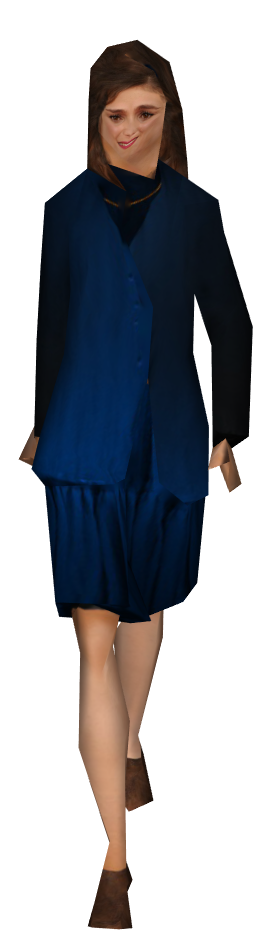
\includegraphics[width=.2\linewidth]{woman/equal_distance/3.png}}
    ~
    \subfloat[Low]{
\includegraphics[width=.2\linewidth]{woman/equal_distance/4.png}}
  \end{figure}
\end{frame}

\begin{frame}{LoD:s (geometry and texture)}
  \begin{figure}
    \subfloat[Super]{\includegraphics[width=.2\linewidth]{woman/cropped/1.png}}
    ~
    \subfloat[High]{
\includegraphics[width=.2\linewidth]{woman/cropped/2.png}}
    ~
    \subfloat[Medium]{
\includegraphics[width=.2\linewidth]{woman/cropped/3.png}}
    ~
    \subfloat[Low]{
\includegraphics[width=.2\linewidth]{woman/cropped/4.png}}
  \end{figure}
\end{frame}

\iffalse

\begin{frame}
  \includegraphics[]{}
\end{frame}

% mesh
\begin{frame}
  \includegraphics[]{}
\end{frame}
\fi



\section*{Summary}

\begin{frame}{Summary}

  \begin{itemize}
  \item
    The \alert{first main message} of your talk in one or two lines.
  \item
    The \alert{second main message} of your talk in one or two lines.
  \item
    Perhaps a \alert{third message}, but not more than that.
  \end{itemize}
  
  % The following outlook is optional.
  \vskip0pt plus.5fill
  \begin{itemize}
  \item
    Outlook
    \begin{itemize}
    \item
      Something you haven't solved.
    \item
      Something else you haven't solved.
    \end{itemize}
  \end{itemize}
\end{frame}


\end{document}


